\documentclass[tikz,border=8pt]{standalone}
\usepackage{amsmath,amssymb}
\usetikzlibrary{arrows.meta,automata,positioning,quotes}
\begin{document}
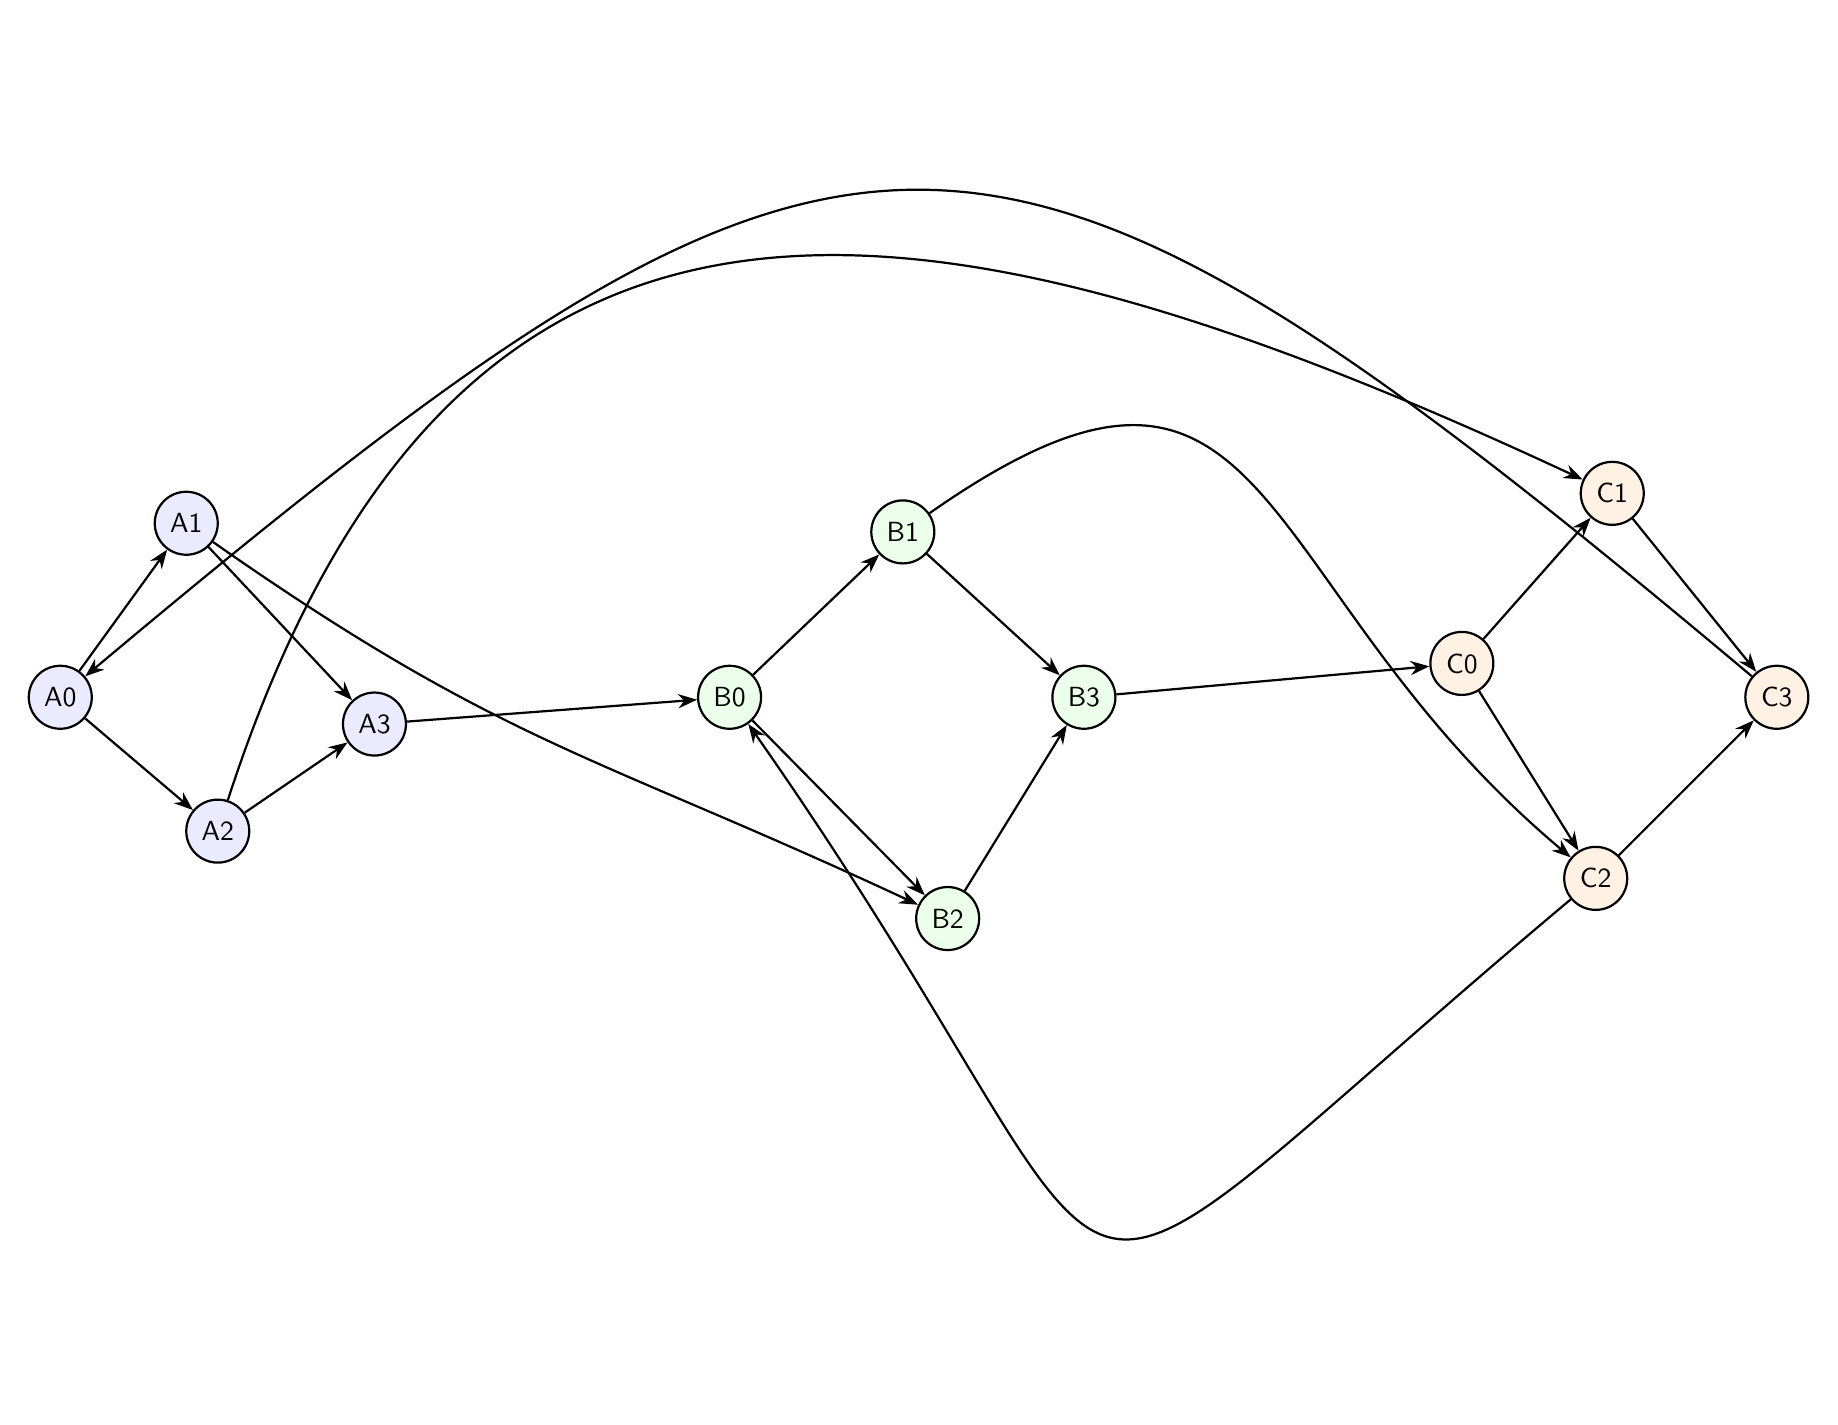
\begin{tikzpicture}[x=1cm,y=1cm]
\tikzset{
  graphnode/.style={circle,draw,thick,minimum size=8mm,inner sep=1pt,font=\sffamily},
  directed/.style={-{Stealth[length=2.4mm]},thick},
  undirected/.style={thick}
}
\node[graphnode,fill=blue!8] (n_A0) at (0.00,0.00) {A0};
\node[graphnode,fill=blue!8] (n_A1) at (1.60,2.21) {A1};
\node[graphnode,fill=blue!8] (n_A2) at (2.00,-1.70) {A2};
\node[graphnode,fill=blue!8] (n_A3) at (3.99,-0.34) {A3};
\node[graphnode,fill=green!8] (n_B0) at (8.50,0.00) {B0};
\node[graphnode,fill=green!8] (n_B1) at (10.70,2.10) {B1};
\node[graphnode,fill=green!8] (n_B2) at (11.27,-2.81) {B2};
\node[graphnode,fill=green!8] (n_B3) at (13.00,0.00) {B3};
\node[graphnode,fill=orange!10] (n_C0) at (17.80,0.43) {C0};
\node[graphnode,fill=orange!10] (n_C1) at (19.71,2.59) {C1};
\node[graphnode,fill=orange!10] (n_C2) at (19.50,-2.30) {C2};
\node[graphnode,fill=orange!10] (n_C3) at (21.80,0.00) {C3};
\draw[directed] (n_A0) -- (n_A1);
\draw[directed] (n_A0) -- (n_A2);
\draw[directed] (n_A1) -- (n_A3);
\draw[directed] (n_A2) -- (n_A3);
\draw[directed] (n_B0) -- (n_B1);
\draw[directed] (n_B0) -- (n_B2);
\draw[directed] (n_B1) -- (n_B3);
\draw[directed] (n_B2) -- (n_B3);
\draw[directed] (n_C0) -- (n_C1);
\draw[directed] (n_C0) -- (n_C2);
\draw[directed] (n_C1) -- (n_C3);
\draw[directed] (n_C2) -- (n_C3);
\draw[directed] (n_A3) -- (n_B0);
\draw[directed] (n_B3) -- (n_C0);
\draw[directed] (n_A1) to[out=-35,in=155,looseness=1.15] (n_B2);
\draw[directed] (n_A2) to[out=72,in=155,looseness=1.35] (n_C1);
\draw[directed] (n_B1) to[out=35,in=140,looseness=1.5] (n_C2);
\draw[directed] (n_C3) to[out=140,in=40,looseness=1.55,dashed] (n_A0);
\draw[directed] (n_C2) to[out=-140,in=-55,looseness=2.35,dashed] (n_B0);
\end{tikzpicture}
\end{document}
